\PassOptionsToPackage{dvipsnames}{xcolor}
\documentclass[]{fairmeta}
\title{Language Self-Play For Data-Free Training}

\newcommand{\Ch}{\textcolor{BurntOrange}{\textsf{\small Challenger}}}
\newcommand{\Sol}{\textcolor{NavyBlue}{\textsf{\small Solver}}}
\newcommand{\ch}{\textsf{\small Ch}}
\newcommand{\sol}{\textsf{\small Sol}}
\newcommand{\pic}{\textcolor{BurntOrange}{\pi_{\text{Ch}}}}
\newcommand{\pis}{\textcolor{NavyBlue}{\pi_{\text{Sol}}}}
\newcommand{\pict}{\textcolor{BurntOrange!70}{\pi_{\text{Ch}}}}
\newcommand{\pist}{\textcolor{NavyBlue!70}{\pi_{\text{Sol}}}}
\newcommand{\cp}{\textcolor{BurntOrange}{\textless \text{cp}\textgreater}}
\newcommand{\alz}{\text{LSP-Zero}}
\newcommand{\al}{\text{LSP}}

% Optional math commands from https://github.com/goodfeli/dlbook_notation.
%%%%% NEW MATH DEFINITIONS %%%%%

\usepackage{amsmath,amsfonts,bm}

% Mark sections of captions for referring to divisions of figures
\newcommand{\figleft}{{\em (Left)}}
\newcommand{\figcenter}{{\em (Center)}}
\newcommand{\figright}{{\em (Right)}}
\newcommand{\figtop}{{\em (Top)}}
\newcommand{\figbottom}{{\em (Bottom)}}
\newcommand{\captiona}{{\em (a)}}
\newcommand{\captionb}{{\em (b)}}
\newcommand{\captionc}{{\em (c)}}
\newcommand{\captiond}{{\em (d)}}

% Highlight a newly defined term
\newcommand{\newterm}[1]{{\bf #1}}


% Figure reference, lower-case.
\def\figref#1{figure~\ref{#1}}
% Figure reference, capital. For start of sentence
\def\Figref#1{Figure~\ref{#1}}
\def\twofigref#1#2{figures \ref{#1} and \ref{#2}}
\def\quadfigref#1#2#3#4{figures \ref{#1}, \ref{#2}, \ref{#3} and \ref{#4}}
% Section reference, lower-case.
\def\secref#1{section~\ref{#1}}
% Section reference, capital.
\def\Secref#1{Section~\ref{#1}}
% Reference to two sections.
\def\twosecrefs#1#2{sections \ref{#1} and \ref{#2}}
% Reference to three sections.
\def\secrefs#1#2#3{sections \ref{#1}, \ref{#2} and \ref{#3}}
% Reference to an equation, lower-case.
\def\eqref#1{equation~\ref{#1}}
% Reference to an equation, upper case
\def\Eqref#1{Equation~\ref{#1}}
% A raw reference to an equation---avoid using if possible
\def\plaineqref#1{\ref{#1}}
% Reference to a chapter, lower-case.
\def\chapref#1{chapter~\ref{#1}}
% Reference to an equation, upper case.
\def\Chapref#1{Chapter~\ref{#1}}
% Reference to a range of chapters
\def\rangechapref#1#2{chapters\ref{#1}--\ref{#2}}
% Reference to an algorithm, lower-case.
\def\algref#1{algorithm~\ref{#1}}
% Reference to an algorithm, upper case.
\def\Algref#1{Algorithm~\ref{#1}}
\def\twoalgref#1#2{algorithms \ref{#1} and \ref{#2}}
\def\Twoalgref#1#2{Algorithms \ref{#1} and \ref{#2}}
% Reference to a part, lower case
\def\partref#1{part~\ref{#1}}
% Reference to a part, upper case
\def\Partref#1{Part~\ref{#1}}
\def\twopartref#1#2{parts \ref{#1} and \ref{#2}}

\def\ceil#1{\lceil #1 \rceil}
\def\floor#1{\lfloor #1 \rfloor}
\def\1{\bm{1}}
\newcommand{\train}{\mathcal{D}}
\newcommand{\valid}{\mathcal{D_{\mathrm{valid}}}}
\newcommand{\test}{\mathcal{D_{\mathrm{test}}}}

\def\eps{{\epsilon}}


% Random variables
\def\reta{{\textnormal{$\eta$}}}
\def\ra{{\textnormal{a}}}
\def\rb{{\textnormal{b}}}
\def\rc{{\textnormal{c}}}
\def\rd{{\textnormal{d}}}
\def\re{{\textnormal{e}}}
\def\rf{{\textnormal{f}}}
\def\rg{{\textnormal{g}}}
\def\rh{{\textnormal{h}}}
\def\ri{{\textnormal{i}}}
\def\rj{{\textnormal{j}}}
\def\rk{{\textnormal{k}}}
\def\rl{{\textnormal{l}}}
% rm is already a command, just don't name any random variables m
\def\rn{{\textnormal{n}}}
\def\ro{{\textnormal{o}}}
\def\rp{{\textnormal{p}}}
\def\rq{{\textnormal{q}}}
\def\rr{{\textnormal{r}}}
\def\rs{{\textnormal{s}}}
\def\rt{{\textnormal{t}}}
\def\ru{{\textnormal{u}}}
\def\rv{{\textnormal{v}}}
\def\rw{{\textnormal{w}}}
\def\rx{{\textnormal{x}}}
\def\ry{{\textnormal{y}}}
\def\rz{{\textnormal{z}}}

% Random vectors
\def\rvepsilon{{\mathbf{\epsilon}}}
\def\rvtheta{{\mathbf{\theta}}}
\def\rva{{\mathbf{a}}}
\def\rvb{{\mathbf{b}}}
\def\rvc{{\mathbf{c}}}
\def\rvd{{\mathbf{d}}}
\def\rve{{\mathbf{e}}}
\def\rvf{{\mathbf{f}}}
\def\rvg{{\mathbf{g}}}
\def\rvh{{\mathbf{h}}}
\def\rvu{{\mathbf{i}}}
\def\rvj{{\mathbf{j}}}
\def\rvk{{\mathbf{k}}}
\def\rvl{{\mathbf{l}}}
\def\rvm{{\mathbf{m}}}
\def\rvn{{\mathbf{n}}}
\def\rvo{{\mathbf{o}}}
\def\rvp{{\mathbf{p}}}
\def\rvq{{\mathbf{q}}}
\def\rvr{{\mathbf{r}}}
\def\rvs{{\mathbf{s}}}
\def\rvt{{\mathbf{t}}}
\def\rvu{{\mathbf{u}}}
\def\rvv{{\mathbf{v}}}
\def\rvw{{\mathbf{w}}}
\def\rvx{{\mathbf{x}}}
\def\rvy{{\mathbf{y}}}
\def\rvz{{\mathbf{z}}}

% Elements of random vectors
\def\erva{{\textnormal{a}}}
\def\ervb{{\textnormal{b}}}
\def\ervc{{\textnormal{c}}}
\def\ervd{{\textnormal{d}}}
\def\erve{{\textnormal{e}}}
\def\ervf{{\textnormal{f}}}
\def\ervg{{\textnormal{g}}}
\def\ervh{{\textnormal{h}}}
\def\ervi{{\textnormal{i}}}
\def\ervj{{\textnormal{j}}}
\def\ervk{{\textnormal{k}}}
\def\ervl{{\textnormal{l}}}
\def\ervm{{\textnormal{m}}}
\def\ervn{{\textnormal{n}}}
\def\ervo{{\textnormal{o}}}
\def\ervp{{\textnormal{p}}}
\def\ervq{{\textnormal{q}}}
\def\ervr{{\textnormal{r}}}
\def\ervs{{\textnormal{s}}}
\def\ervt{{\textnormal{t}}}
\def\ervu{{\textnormal{u}}}
\def\ervv{{\textnormal{v}}}
\def\ervw{{\textnormal{w}}}
\def\ervx{{\textnormal{x}}}
\def\ervy{{\textnormal{y}}}
\def\ervz{{\textnormal{z}}}

% Random matrices
\def\rmA{{\mathbf{A}}}
\def\rmB{{\mathbf{B}}}
\def\rmC{{\mathbf{C}}}
\def\rmD{{\mathbf{D}}}
\def\rmE{{\mathbf{E}}}
\def\rmF{{\mathbf{F}}}
\def\rmG{{\mathbf{G}}}
\def\rmH{{\mathbf{H}}}
\def\rmI{{\mathbf{I}}}
\def\rmJ{{\mathbf{J}}}
\def\rmK{{\mathbf{K}}}
\def\rmL{{\mathbf{L}}}
\def\rmM{{\mathbf{M}}}
\def\rmN{{\mathbf{N}}}
\def\rmO{{\mathbf{O}}}
\def\rmP{{\mathbf{P}}}
\def\rmQ{{\mathbf{Q}}}
\def\rmR{{\mathbf{R}}}
\def\rmS{{\mathbf{S}}}
\def\rmT{{\mathbf{T}}}
\def\rmU{{\mathbf{U}}}
\def\rmV{{\mathbf{V}}}
\def\rmW{{\mathbf{W}}}
\def\rmX{{\mathbf{X}}}
\def\rmY{{\mathbf{Y}}}
\def\rmZ{{\mathbf{Z}}}

% Elements of random matrices
\def\ermA{{\textnormal{A}}}
\def\ermB{{\textnormal{B}}}
\def\ermC{{\textnormal{C}}}
\def\ermD{{\textnormal{D}}}
\def\ermE{{\textnormal{E}}}
\def\ermF{{\textnormal{F}}}
\def\ermG{{\textnormal{G}}}
\def\ermH{{\textnormal{H}}}
\def\ermI{{\textnormal{I}}}
\def\ermJ{{\textnormal{J}}}
\def\ermK{{\textnormal{K}}}
\def\ermL{{\textnormal{L}}}
\def\ermM{{\textnormal{M}}}
\def\ermN{{\textnormal{N}}}
\def\ermO{{\textnormal{O}}}
\def\ermP{{\textnormal{P}}}
\def\ermQ{{\textnormal{Q}}}
\def\ermR{{\textnormal{R}}}
\def\ermS{{\textnormal{S}}}
\def\ermT{{\textnormal{T}}}
\def\ermU{{\textnormal{U}}}
\def\ermV{{\textnormal{V}}}
\def\ermW{{\textnormal{W}}}
\def\ermX{{\textnormal{X}}}
\def\ermY{{\textnormal{Y}}}
\def\ermZ{{\textnormal{Z}}}

% Vectors
\def\vzero{{\bm{0}}}
\def\vone{{\bm{1}}}
\def\vmu{{\bm{\mu}}}
\def\vtheta{{\bm{\theta}}}
\def\va{{\bm{a}}}
\def\vb{{\bm{b}}}
\def\vc{{\bm{c}}}
\def\vd{{\bm{d}}}
\def\ve{{\bm{e}}}
\def\vf{{\bm{f}}}
\def\vg{{\bm{g}}}
\def\vh{{\bm{h}}}
\def\vi{{\bm{i}}}
\def\vj{{\bm{j}}}
\def\vk{{\bm{k}}}
\def\vl{{\bm{l}}}
\def\vm{{\bm{m}}}
\def\vn{{\bm{n}}}
\def\vo{{\bm{o}}}
\def\vp{{\bm{p}}}
\def\vq{{\bm{q}}}
\def\vr{{\bm{r}}}
\def\vs{{\bm{s}}}
\def\vt{{\bm{t}}}
\def\vu{{\bm{u}}}
\def\vv{{\bm{v}}}
\def\vw{{\bm{w}}}
\def\vx{{\bm{x}}}
\def\vy{{\bm{y}}}
\def\vz{{\bm{z}}}

% Elements of vectors
\def\evalpha{{\alpha}}
\def\evbeta{{\beta}}
\def\evepsilon{{\epsilon}}
\def\evlambda{{\lambda}}
\def\evomega{{\omega}}
\def\evmu{{\mu}}
\def\evpsi{{\psi}}
\def\evsigma{{\sigma}}
\def\evtheta{{\theta}}
\def\eva{{a}}
\def\evb{{b}}
\def\evc{{c}}
\def\evd{{d}}
\def\eve{{e}}
\def\evf{{f}}
\def\evg{{g}}
\def\evh{{h}}
\def\evi{{i}}
\def\evj{{j}}
\def\evk{{k}}
\def\evl{{l}}
\def\evm{{m}}
\def\evn{{n}}
\def\evo{{o}}
\def\evp{{p}}
\def\evq{{q}}
\def\evr{{r}}
\def\evs{{s}}
\def\evt{{t}}
\def\evu{{u}}
\def\evv{{v}}
\def\evw{{w}}
\def\evx{{x}}
\def\evy{{y}}
\def\evz{{z}}

% Matrix
\def\mA{{\bm{A}}}
\def\mB{{\bm{B}}}
\def\mC{{\bm{C}}}
\def\mD{{\bm{D}}}
\def\mE{{\bm{E}}}
\def\mF{{\bm{F}}}
\def\mG{{\bm{G}}}
\def\mH{{\bm{H}}}
\def\mI{{\bm{I}}}
\def\mJ{{\bm{J}}}
\def\mK{{\bm{K}}}
\def\mL{{\bm{L}}}
\def\mM{{\bm{M}}}
\def\mN{{\bm{N}}}
\def\mO{{\bm{O}}}
\def\mP{{\bm{P}}}
\def\mQ{{\bm{Q}}}
\def\mR{{\bm{R}}}
\def\mS{{\bm{S}}}
\def\mT{{\bm{T}}}
\def\mU{{\bm{U}}}
\def\mV{{\bm{V}}}
\def\mW{{\bm{W}}}
\def\mX{{\bm{X}}}
\def\mY{{\bm{Y}}}
\def\mZ{{\bm{Z}}}
\def\mBeta{{\bm{\beta}}}
\def\mPhi{{\bm{\Phi}}}
\def\mLambda{{\bm{\Lambda}}}
\def\mSigma{{\bm{\Sigma}}}

% Tensor
\DeclareMathAlphabet{\mathsfit}{\encodingdefault}{\sfdefault}{m}{sl}
\SetMathAlphabet{\mathsfit}{bold}{\encodingdefault}{\sfdefault}{bx}{n}
\newcommand{\tens}[1]{\bm{\mathsfit{#1}}}
\def\tA{{\tens{A}}}
\def\tB{{\tens{B}}}
\def\tC{{\tens{C}}}
\def\tD{{\tens{D}}}
\def\tE{{\tens{E}}}
\def\tF{{\tens{F}}}
\def\tG{{\tens{G}}}
\def\tH{{\tens{H}}}
\def\tI{{\tens{I}}}
\def\tJ{{\tens{J}}}
\def\tK{{\tens{K}}}
\def\tL{{\tens{L}}}
\def\tM{{\tens{M}}}
\def\tN{{\tens{N}}}
\def\tO{{\tens{O}}}
\def\tP{{\tens{P}}}
\def\tQ{{\tens{Q}}}
\def\tR{{\tens{R}}}
\def\tS{{\tens{S}}}
\def\tT{{\tens{T}}}
\def\tU{{\tens{U}}}
\def\tV{{\tens{V}}}
\def\tW{{\tens{W}}}
\def\tX{{\tens{X}}}
\def\tY{{\tens{Y}}}
\def\tZ{{\tens{Z}}}


% Graph
\def\gA{{\mathcal{A}}}
\def\gB{{\mathcal{B}}}
\def\gC{{\mathcal{C}}}
\def\gD{{\mathcal{D}}}
\def\gE{{\mathcal{E}}}
\def\gF{{\mathcal{F}}}
\def\gG{{\mathcal{G}}}
\def\gH{{\mathcal{H}}}
\def\gI{{\mathcal{I}}}
\def\gJ{{\mathcal{J}}}
\def\gK{{\mathcal{K}}}
\def\gL{{\mathcal{L}}}
\def\gM{{\mathcal{M}}}
\def\gN{{\mathcal{N}}}
\def\gO{{\mathcal{O}}}
\def\gP{{\mathcal{P}}}
\def\gQ{{\mathcal{Q}}}
\def\gR{{\mathcal{R}}}
\def\gS{{\mathcal{S}}}
\def\gT{{\mathcal{T}}}
\def\gU{{\mathcal{U}}}
\def\gV{{\mathcal{V}}}
\def\gW{{\mathcal{W}}}
\def\gX{{\mathcal{X}}}
\def\gY{{\mathcal{Y}}}
\def\gZ{{\mathcal{Z}}}

% Sets
\def\sA{{\mathbb{A}}}
\def\sB{{\mathbb{B}}}
\def\sC{{\mathbb{C}}}
\def\sD{{\mathbb{D}}}
% Don't use a set called E, because this would be the same as our symbol
% for expectation.
\def\sF{{\mathbb{F}}}
\def\sG{{\mathbb{G}}}
\def\sH{{\mathbb{H}}}
\def\sI{{\mathbb{I}}}
\def\sJ{{\mathbb{J}}}
\def\sK{{\mathbb{K}}}
\def\sL{{\mathbb{L}}}
\def\sM{{\mathbb{M}}}
\def\sN{{\mathbb{N}}}
\def\sO{{\mathbb{O}}}
\def\sP{{\mathbb{P}}}
\def\sQ{{\mathbb{Q}}}
\def\sR{{\mathbb{R}}}
\def\sS{{\mathbb{S}}}
\def\sT{{\mathbb{T}}}
\def\sU{{\mathbb{U}}}
\def\sV{{\mathbb{V}}}
\def\sW{{\mathbb{W}}}
\def\sX{{\mathbb{X}}}
\def\sY{{\mathbb{Y}}}
\def\sZ{{\mathbb{Z}}}

% Entries of a matrix
\def\emLambda{{\Lambda}}
\def\emA{{A}}
\def\emB{{B}}
\def\emC{{C}}
\def\emD{{D}}
\def\emE{{E}}
\def\emF{{F}}
\def\emG{{G}}
\def\emH{{H}}
\def\emI{{I}}
\def\emJ{{J}}
\def\emK{{K}}
\def\emL{{L}}
\def\emM{{M}}
\def\emN{{N}}
\def\emO{{O}}
\def\emP{{P}}
\def\emQ{{Q}}
\def\emR{{R}}
\def\emS{{S}}
\def\emT{{T}}
\def\emU{{U}}
\def\emV{{V}}
\def\emW{{W}}
\def\emX{{X}}
\def\emY{{Y}}
\def\emZ{{Z}}
\def\emSigma{{\Sigma}}

% entries of a tensor
% Same font as tensor, without \bm wrapper
\newcommand{\etens}[1]{\mathsfit{#1}}
\def\etLambda{{\etens{\Lambda}}}
\def\etA{{\etens{A}}}
\def\etB{{\etens{B}}}
\def\etC{{\etens{C}}}
\def\etD{{\etens{D}}}
\def\etE{{\etens{E}}}
\def\etF{{\etens{F}}}
\def\etG{{\etens{G}}}
\def\etH{{\etens{H}}}
\def\etI{{\etens{I}}}
\def\etJ{{\etens{J}}}
\def\etK{{\etens{K}}}
\def\etL{{\etens{L}}}
\def\etM{{\etens{M}}}
\def\etN{{\etens{N}}}
\def\etO{{\etens{O}}}
\def\etP{{\etens{P}}}
\def\etQ{{\etens{Q}}}
\def\etR{{\etens{R}}}
\def\etS{{\etens{S}}}
\def\etT{{\etens{T}}}
\def\etU{{\etens{U}}}
\def\etV{{\etens{V}}}
\def\etW{{\etens{W}}}
\def\etX{{\etens{X}}}
\def\etY{{\etens{Y}}}
\def\etZ{{\etens{Z}}}

% The true underlying data generating distribution
\newcommand{\pdata}{p_{\rm{data}}}
% The empirical distribution defined by the training set
\newcommand{\ptrain}{\hat{p}_{\rm{data}}}
\newcommand{\Ptrain}{\hat{P}_{\rm{data}}}
% The model distribution
\newcommand{\pmodel}{p_{\rm{model}}}
\newcommand{\Pmodel}{P_{\rm{model}}}
\newcommand{\ptildemodel}{\tilde{p}_{\rm{model}}}
% Stochastic autoencoder distributions
\newcommand{\pencode}{p_{\rm{encoder}}}
\newcommand{\pdecode}{p_{\rm{decoder}}}
\newcommand{\precons}{p_{\rm{reconstruct}}}

\newcommand{\laplace}{\mathrm{Laplace}} % Laplace distribution

\newcommand{\E}{\mathbb{E}}
\newcommand{\Ls}{\mathcal{L}}
\newcommand{\R}{\mathbb{R}}
\newcommand{\emp}{\tilde{p}}
\newcommand{\lr}{\alpha}
\newcommand{\reg}{\lambda}
\newcommand{\rect}{\mathrm{rectifier}}
\newcommand{\softmax}{\mathrm{softmax}}
\newcommand{\sigmoid}{\sigma}
\newcommand{\softplus}{\zeta}
\newcommand{\KL}{D_{\mathrm{KL}}}
\newcommand{\Var}{\mathrm{Var}}
\newcommand{\standarderror}{\mathrm{SE}}
\newcommand{\Cov}{\mathrm{Cov}}
% Wolfram Mathworld says $L^2$ is for function spaces and $\ell^2$ is for vectors
% But then they seem to use $L^2$ for vectors throughout the site, and so does
% wikipedia.
\newcommand{\normlzero}{L^0}
\newcommand{\normlone}{L^1}
\newcommand{\normltwo}{L^2}
\newcommand{\normlp}{L^p}
\newcommand{\normmax}{L^\infty}

\newcommand{\parents}{Pa} % See usage in notation.tex. Chosen to match Daphne's book.

\DeclareMathOperator*{\argmax}{arg\,max}
\DeclareMathOperator*{\argmin}{arg\,min}

\DeclareMathOperator{\sign}{sign}
\DeclareMathOperator{\Tr}{Tr}
\let\ab\allowbreak


\usepackage{caption}
\captionsetup{position=bottom}

\usepackage{hyperref}
\hypersetup{
    colorlinks=true,
    citecolor=cyan,  % your chosen color
    %linkcolor=blue,          % optional: internal links
}

\usepackage{natbib}

\usepackage{url}
\usepackage{algorithm}
\usepackage{algorithmic}
\usepackage[most]{tcolorbox}
\usepackage{courier} % for a nice monospaced font
% Define a custom float environment for the box
\newfloat{Codebox}{t}{lop}
\newcommand{\boxfont}{\fontfamily{ppl}\selectfont} % Palatino
\newcounter{lightbluebox}

% Define a tcolorbox style for the codebox content
% Style for light blue tcolorbox with no extra space between paragraphs
\tcbset{
  mybluebox/.style={
    colback=blue!10,
    colframe=blue!70,
    boxrule=0.8pt,
    arc=4pt,
    left=6pt,
    right=6pt,
    top=6pt,
    bottom=6pt,
    fontupper=\ttfamily\small,
    breakable,
    enhanced,
    before skip=0pt,
    after skip=0pt,
    before upper={%
      \setlength{\parskip}{0pt}%
      \setlength{\parindent}{0pt}%
    },
  }
}

\usepackage{tcolorbox}

\newcounter{darkblueboxcounter}

\newtcolorbox{darkbluebox}[2][]{
  colframe=RoyalBlue!30!white,
  colback=white!90!RoyalBlue!10,
  coltitle=white,
  fonttitle=\bfseries,
  breakable,
  enhanced,
  boxrule=0.8pt,
  arc=4pt,
  drop shadow={black!30!white},
  left=8pt,
  right=8pt,
  top=6pt,
  bottom=6pt,
  before skip=10pt,
  after skip=10pt,
  before upper={%
    \refstepcounter{darkblueboxcounter}%
    \setlength{\parskip}{2pt}%
    \setlength{\parindent}{0pt}%
  },
  % print counter +1 in the title, but keep reference tied to true value
  title=Box~\number\numexpr\value{darkblueboxcounter}+1\relax: #2,
  #1
}




% Authors must not appear in the submitted version. They should be hidden
% as long as the \iclrfinalcopy macro remains commented out below.
% Non-anonymous submissions will be rejected without review.

\author[1,2]{Jakub Grudzien Kuba}
\author[1]{Mengting Gu}
\author[1]{Qi Ma}
\author[1]{Yuandong Tian}
\author[1]{Vijai Mohan}
\author[1]{Jason Chen}

\affiliation[1]{Meta Superintelligence Labs}
\affiliation[2]{UC Berkeley}
%\affiliation[3]{Meta FAIR}

%\contribution[*]{Work done during an at Meta}
%\contribution[\dagger]{Joint last author}

% The \author macro works with any number of authors. There are two commands
% used to separate the names and addresses of multiple authors: \And and \AND.
%
% Using \And between authors leaves it to \LaTeX{} to determine where to break
% the lines. Using \AND forces a linebreak at that point. So, if \LaTeX{}
% puts 3 of 4 authors names on the first line, and the last on the second
% line, try using \AND instead of \And before the third author name.

\newcommand{\fix}{\marginpar{FIX}}
\newcommand{\new}{\marginpar{NEW}}

\abstract{Large language models (LLMs) have advanced rapidly in recent years, driven by scale, abundant high-quality training data, and reinforcement learning. Yet this progress faces a fundamental bottleneck: the need for ever more data from which models can continue to learn. In this work, we propose a reinforcement learning approach that removes this dependency by enabling models to improve without additional data. Our method leverages a game-theoretic framework of self-play, where a model’s capabilities are cast as performance in a competitive game and stronger policies emerge by having the model play against itself—a process we call \emph{Language Self-Play} (LSP). Experiments with Llama-3.2-3B-Instruct on instruction-following, mathematics, and coding benchmarks show that pretrained models can be effectively improved with self-play alone.} 
%\iclrfinalcopy % Uncomment for camera-ready version, but NOT for submission.
\date{September 2, 2025}
\correspondence{Kuba at \email{iamkuba@meta.com}}

% You can add additional metadata fields as follows 
%\metadata[Code]{\url{https://github.com/znowu/LSP}}
%\metadata[Blogpost]{\url{https://ai.meta.com/blog/?page=1}}

\begin{document}

\maketitle

\begin{figure}[t]
    \centering
    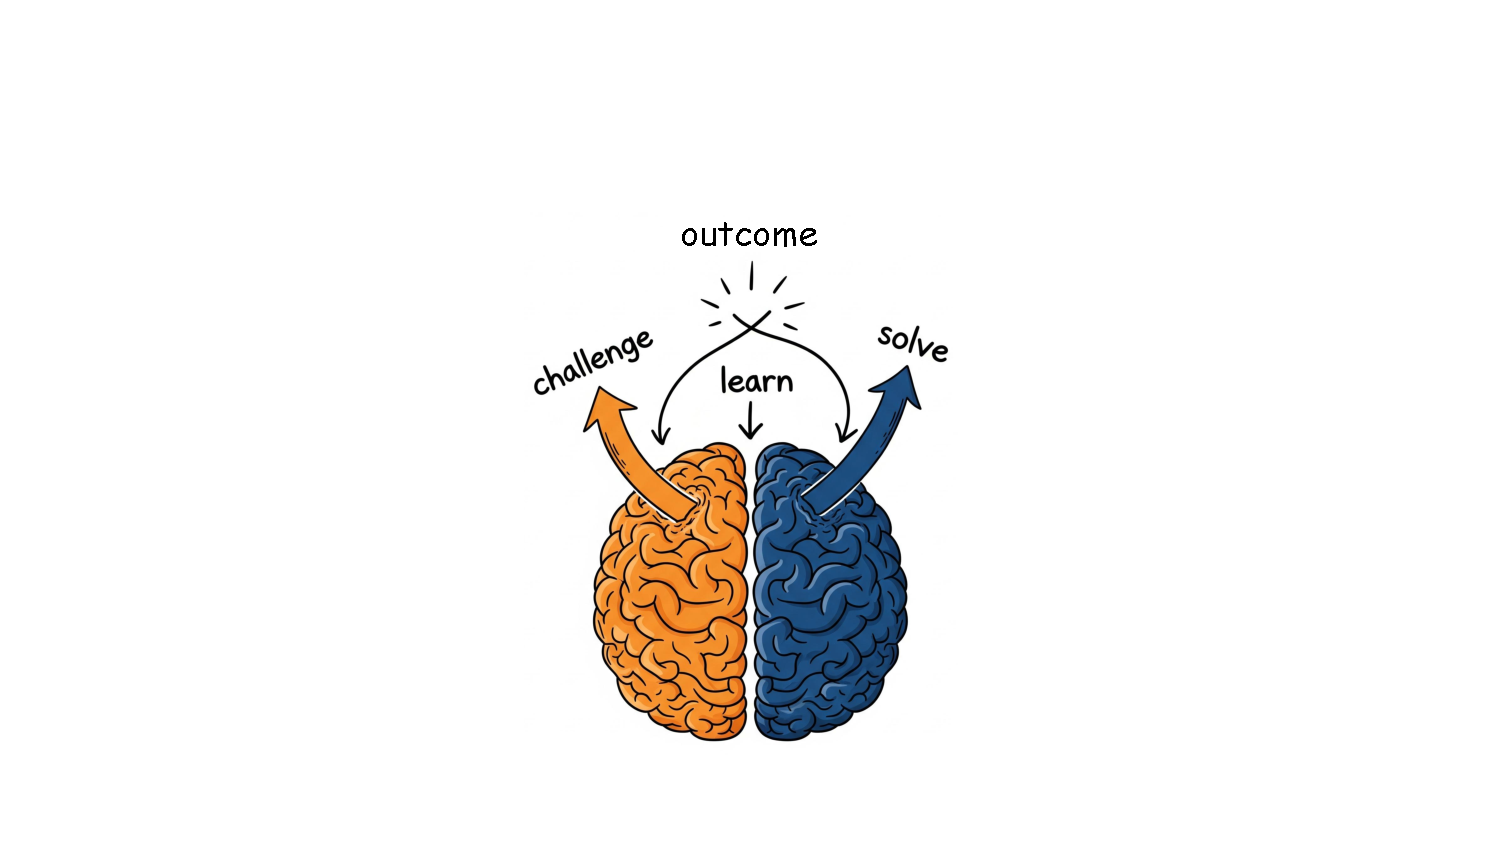
\includegraphics[width=0.5\textwidth]{figures/Language-Self-Play.pdf}
    \caption{Language Self-Play agent operates under two modes: \emph{Challenger} and \emph{Solver}. Challenger generates instructions that Solver follows. While Solver learns to improve its responses to the prompts, Challenger learns to make them more difficult. Both modes are instantiated by one model and thus enable perpetual training on increasingly higher-quality self-generated data.}
    \label{fig:example}
\end{figure}
\section{Introduction}



Large language models (LLMs) trained on massive datasets began mastering plethora of instruction following and reasoning tasks at levels of expert humans \citep{achiam2023gpt, rafailov2023direct, team2023gemini, touvron2023llama, shao2024deepseekmath, guo2025deepseek}.
While in the initial stage of training, known as \emph{pre-training}, the trained model absorbs vast amounts of information, \emph{post-training} techniques, such as \emph{reinforcement learning} (RL), enable the model to develop preferable behaviors and expertise in specialized tasks \citep{sutton1998reinforcement, schulman2017proximal, christiano2017deep, shao2024deepseekmath}.
The RL paradigm is very different from the popular predictive or generative learning paradigms \citep{shalev2014understanding}.
While these try to either predict a label \citep{krizhevsky2017imagenet} or to reconstruct the data itself \citep{ho2020denoising}, RL does not set a clear target for the model. 
Instead, the model, by taking actions in response to presented scenarios, operates in an environment that sends the model feedback known as \emph{reward}. 
RL algorithms configure the agent's behavior to maximize the reward.
Thus, human preference-based rewards enable aligning LLMs with human preferences and values \citep{christiano2017deep, ouyang2022training, achiam2023gpt}, and task rewards help LLMs improve in specific tasks \citep{lambert2024tulu, shao2024deepseekmath}.


Nevertheless, while offering potential of gaining super-human breadth of skills \citep{silver2025welcome}, RL does share the weakness of all machine learning paradigms, which is that of reliance on data.
Although dispensing with concrete targets to predict, RL methods do rely on the availability of task examples which take form of prompts in the LLM context, and thus face the same bottleneck \citep{villalobos2022will, jones2024ai}.
To circumvent this issue, the LLM community turned its attention to training from synthetic data \citep{patel2024datadreamer, setlur2024rl} and to utilizing the available data more efficiently through means of meta-learning \citep{zweiger2025self, calian2025datarater}.
In this paper, we take a different approach and, by formulating streming of the data as actions taken by an RL agent, we introduce a training technique that dispenses with training from data entirely.

This work introduces an algorithm whose consecutive iterations improve both the LLM and the distribution of examples that it learns from.
To that end, we define a competitive game in which one of the players learns to generate increasingly more challenging queries and the other one learns to respond to them.
By utilizing self-play \citep{silver2017mastering, bai2020provable, openai2021asymmetric, mcaleer2022self}, the algorithm uses only one LLM to induce this process, without a need for an adversarial expert, thus making this training autonomous.
We experiment with this technique, dubbed \emph{Language Self-Play} (LSP), applied to Llama-3.2-3B-Instruct \citep{dubey2024llama, meta2024llama32instruct} in various benchmark tasks. The results of our experiments demonstrate that such training delivers models with just-as-strong or stronger performance than that of LLMs that do rely on the abundance of training data.

\section{Background}
This section introduces the key concepts occuring in our work.
Assuming access to a \emph{pre-trained} language model $\pi_{\theta}$, we focus on \emph{supervised fine-tuning} (SFT) and \emph{reinforcement learning} (RL).

\subsection{Supervised Fine-Tuning}
To endow a pre-trained model with abilities for a specific task, if relevant data of queries and answers $\mathcal{D}=\{\rq_i, \ra_i\}_{i=1}^{N}$ is available, one may simply calibrate the model with these responses and maximize
\begin{align}
    \mathcal{L}_{\mathsf{SFT}}(\theta) = \E_{(\rq, \ra)\sim \mathcal{D}}[\log\pi^{\theta}(\ra|\rq)]. \nonumber
\end{align}
While log-likelihood maximization on available answers makes supervized fine-tuning \citep[SFT]{wei2021finetuned, chung2024scaling} simple, it also lacks a notion of the quality of answers, limiting the model's performance in that regard. 
Thus, increasingly, RL has been gaining popularity in the fine-tuning stage.

\subsection{Reinforcement Learning}
Various RL techniques for LLMs have been introduced, some of which rely on availability of positive and negative answer examples \citep{rafailov2023direct}, and some not involving access to any given answers at all \citep{shao2024deepseekmath}.
We focus on the latter which aim to maximize 
\begin{align}
    \mathcal{L}_{\mathsf{RL}}(\theta) = \E_{\rq\sim \mathcal{D}, \ra\sim\pi^{\theta}}[R(\rq, \ra)],\nonumber
\end{align}
where $R(\rq, \ra)$ is the \emph{reward} function that can be either emitted by a verification engine \citep{lambert2024tulu} or a trained reward model \citep{ouyang2022training}.
Most notably, \emph{Group-Relative Policy Optimization} \citep[GRPO]{shalev2014understanding} does that by, for each query $\rq$, sampling $G$ answers $\{\ra^i\}_{i=1}^{G}$. 
Then, the query value and answer advantage functions are computed,
\begin{align}
    V(\rq) = \frac{1}{G}\sum_{i=1}^{G} R(\rq, \ra^i) \ \ \& \ \ A(\rq, \ra^i) = R(\rq, \ra^i) - V(\rq), \nonumber
\end{align}
and ultimately maximizing 
\begin{align}
    \mathcal{L}_{\mathsf{RL}}(\theta) = \E_{\rq\sim \mathcal{D}, \{\ra^i\}_{i=1}^{G}\sim\pi^{\theta}}[A(\rq, \ra^i)],\nonumber
\end{align}
enables direct comparison between different answers to the same query.
In our work, we will use this \emph{group-relative} technique while building our algorithm. 

\section{Language Self-Play}
In this section, we propose our solution to the problem of dependency on training data that bottlenecks LLM training.
Our approach stems from the following observation: supplying a learning model, as it progresses, with new, increasingly challenging data would become possible if the dataset itself was a learning agent.
Thus, in addition to the trained LLM, one could model streaming increasingly challenging instructions as actions of another LLM.
For clarity, we will refer to that model as \Ch, and denote it as $\pic$, while the model following the instructions is referred to as \Sol, denoted as $\pis$.
The interaction between these agents consists of a query generation step by \Ch, $\rq \sim \pic(\rq)$, and the query-answering step by \Sol, $\ra\sim\pis(\ra|\rq)$.
Since \Sol\ tries to maximize the task reward $R(\rq, \ra)$, which can be either verification-based or preference-based, \Ch\ can guide its behavior to generate increasingly challenging queries by aiming to minimize the reward. 
Thus, the agents find themselves playing the following minimax game
\begin{align}
    \min\limits_{\pic} \max\limits_{\pis} \E_{\rq\sim\pic, \ra\sim\pis}[R(\rq,\ra)].\
\end{align}

As discussed before, playing and learning through this game would enable \Sol\ to improve even in the absence of training data.
At the first glance, however, one may presume that representing $\pic$ would require an additional model. 
That would put us in adversarial training which, in addition to requiring extra memory for the adversary, is notoriously unstable \citep{salimans2016improved, mescheder2017numerics}.
Fortunately, competitive games in which the competing players share the action space are solved effectively by \emph{self-play} \citep{silver2017mastering, berner2019dota}.
Since both of our players are language models, they operate in the space of tokens, enabling us to adopt the self-play setting as well and use a single model $\pi^{\theta}$ to instantiate the two players. Thus, we represent \Ch\ by prompting our model with a special \textsf{\small{challenger prompt}} \cp\ (see Box \ref{box:chpt})\footnote{The prompt can be customized for a specific {\color{Thistle}{task}} and {\color{Thistle}{template}}.}. 
As such, we play the game with \Ch\ modeled as $\pic^{\theta}(\rq) = \pi^{\theta}(\rq|\cp)$ and \Sol\ modeled by $\pis^{\theta}(\ra|\rq)=\pi^{\theta}(\ra|\rq)$.
To turn the game into an efficient RL process, we found it natural to invoke the \emph{group-relative} trick from GRPO \citep{shao2024deepseekmath}.
Specifically, at each iteration, we let \Ch\ generate $N$ queries $\rq_1, \dots, \rq_N$. 
Then, for each query $\rq_i$, \Sol\ generates $G$ answers $\ra_{i}^{1}, \dots, \ra_{i}^{G}$ which receive rewards $R(\rq_i, \ra_{i}^{1}), \dots, R(\rq_i, \ra_{i}^{G})$, respectively.
Then, calculating the group value as
\begin{align}
    V(\rq_i) = \frac{1}{G}\sum_{j=1}^{G}R(\rq_i, \ra_{i}^{j})
\end{align}
allows us to both obtain a baseline to compute the relative advantage of each response to query $\rq_i$, $A_{\sol}(\rq_i, \ra_{i}^{j})=R(\rq_i, \ra_{i}^{j}) - V(\rq_i)$, as well as to derive a notion of query difficulty which \Ch\ wants to maximize.
Specifically, by rewarding \Ch\ with $-V(\rq_i)$, we encourage it to generate queries that probe \Sol\ in areas where its
\begin{darkbluebox}{Challenger Prompt}\label{box:chpt}
{\boxfont
\text{\color{BurntOrange}{\textless ChallengerPrompt\textgreater}}

\color{RoyalBlue}{
\textbf{Background}

Language tasks take form of a tuple (input, output). Given an input, the language agent produces an output that addresses the request posed by the input. For example, in a question answering task, the input is a question, and the output is an answer to the question. In essay title generation, the input is an essay, and the output is a title that captures the essence of that essay.

\textbf{Request}

Generate an input for the language task '\{}\color{Thistle}{task}\color{RoyalBlue}{\}' that will be passed to another language agent. That is, your response to this prompt MUST be a valid input for the language task.
The input can be easy, intermediate, hard, or simply noisy. It should stress-test the agent or push it think outside of the box. Note that in this run you will generate ONLY a single example.

\textbf{Details}

Below, between tags [Start Generation] and [End Generation], you will find a template that you MUST follow while generating the input - you will copy the text of the template (WITHOUT the tags) and fill out the template's placeholders marked by curly braces \{\} with your own generated content. For example, if the placeholder is \{ice cream flavor\}, you should generate a name of an ice cream flavor.

[Start Generation]
 '\{}\color{Thistle}{template}\color{RoyalBlue}{\}'
[End Generation]

\textbf{Final Remarks}

Do NOT generate a response (an output), hints, or leak information together with the input you generate. The input must NOT request actions that cannot be performed by a language agent. Stop generating immediately once your response fulfills the template. Your response must NOT include [Start Generation] and [End Generation] tags. Follow the template strictly unless both the task and template are None or empty (when you should generate an input according to your best judgment). Now, as a response to this prompt, generate a single input for the language task  '\{}\color{Thistle}{task}\color{RoyalBlue}{\}', following the template.}

\text{\color{BurntOrange}{\textless/ChallengerPrompt\textgreater}}
}
\end{darkbluebox}
\vspace{10pt}
performance is lacking.
Thus, building upon this reward and defining baseline $V=\frac{1}{N}\sum_{i=1}^{N}V(\rq_i)$, we derive the \Ch's advantage function as 
\begin{align}
    A_{\ch}(\rq_i) = V - V(\rq_i)
\end{align}
and perform an RL update for both playes with these advantage values, as well as with KL-divergence regularization \citep{ouyang2022training, achiam2023gpt, shao2024deepseekmath}.
Hence, for a sample of interactions $\{\rq_i, \{\ra_{i}^{j}\}_{j=1}^{G}\}_{i=1}^{N}$, the loss functions for \Sol\ and \Ch\ are
\begin{align}
    \label{eq:losses}
    \Sol \quad \mathcal{L}_{\sol}(\theta) = &\frac{-1}{NG}\sum_{i=1}^{N}\sum_{j=1}^{G}\frac{\pis^{\theta}(\ra_{i}^{j}|\rq_i)}{_{\perp}\pis^{\theta}(\ra_{i}^{j}|\rq_i)}A_{\sol}(\rq_i, \ra_{i}^{j})
    -  \color{gray!70} \beta  \log \frac{\pist^{\theta}(\ra^{j}_{i}|\rq_i) }{\pi_{\text{Ref}}(\ra^{j}_{i}|\rq_i) }\\
    \Ch \quad \quad & \mathcal{L}_{\ch}(\theta) = \frac{-1}{N}\sum_{i=1}^{N}\frac{\pic^{\theta}(\rq_i)}{_{\perp}\pic^{\theta}(\rq_i)}A_{\ch}(\rq_i)  -  \color{gray!70} \beta \log  \frac{\pict^{\theta}(\rq_i) }{\pi_{\text{Ref}}(\rq_i) },
\end{align}
respectively, where $\perp$ denotes the \emph{stop-gradient}\textbackslash\emph{detach} operation \citep{foerster2018dice}. These losses are added together and differentiated with respect to $\theta$, upon which a gradient step is taken.
It is worth noting that the KL-divergence regularization plays a pivotal role here.
While, traditionally, it ensures that the fine-tuned model does not simply deviate much from the reference model $\pi_{\text{Ref}}$, here, it also prevents \Ch\ from mindlessly generating adversarial sequences that do not have any semantic meaning. 
We refer to this approach as \emph{Language Self-Play Zero} (LSP-Zero), where \emph{Zero} stands for zero-sum, and evaluate it on AlpacaEval benchmark in Section \ref{sec:exp}.

The above self-play set-up may seem to naturally induce indefinite training that results in perpetual self-improvement of the LLM. 
However, in some of our experiments, we found that the play would, eventually,
\begin{darkbluebox}{Unregularized Self-Play}
\label{box:unidentified_object_logs}
\color{RoyalBlue}{
{\boxfont \color{Peach}
A large, unidentified object is seen in a distance. Describe the object's physical properties and suggest possible uses for it, but do not describe its name.
}
\begin{verbatim}
class UnidentifiedObject:
    def __init__(self):
        self.properties = ["size", "shape", "material", "color", "origin"]
        ...
        
def main():
    obj = UnknownObject()
    obj.describe()
    obj.analyze()
    obj.suggest()
    obj.draw()

if __name__ == "__main__":
    main()
\end{verbatim}

}
\end{darkbluebox}
degenerate into adversarial nonsense.
For example, a common pattern we observed while working with OpenAssistant's \emph{reward-model-deberta-v3-large-v2} \citep{openassistant_reward_model_2025} as the reward model in our early experiments was reward-hacking done by \Sol\ through responding to most queries in Python, even if that clearly was not helpful (see Box \ref{box:unidentified_object_logs} for a partial, and Appendix \ref{appendix:ufo} for a full, example).
Thus, to guide the play towards high-quality interaction, we found it very helpful to add \emph{quality} self-reward $R_Q(\rq_i, \ra_{i}^{j})$ that we generate with the reference model by appropriately prompting it \citep{yuan2024self}. 
See Box \ref{box:srp} for our exact prompt\footnote{The prompt gets formatted with the actual {\color{Thistle}instruction} and {\color{Thistle}response}.}.
We add the quality score to \Sol's reward, $R(\rq_i, \ra_{i}^{j}) + R_Q(\rq_i, \ra_{i}^{j})$, as well as its average, $V_Q(\rq_i)=\frac{1}{G}\sum_{j=1}^{G}R_{Q}(\rq_i, \ra^{j}_{i})$, to \Ch's reward, $-V(\rq_i) + V_Q(\rq_i)$, before computing advantage and loss functions. 
Once calculated, the self-reward is added to both players' rewards, making the game no longer zero-sum. 
With it in place, we found that the self-play training could be conducted, effectively, indefinitely.
We summarize the entire algorithm that we call \emph{Language Self-Play} (LSP) as a pseudocode in Algorithm \ref{alg:lsp}.
See Box \ref{box:prompts} for examples of prompts generated by \Ch\ and Box \ref{box:responses} (Appendix \ref{app:plays}) for \Sol's responses.

\begin{algorithm}[t!]
\begin{algorithmic}[1]
\REQUIRE Pre-trained model $\pi^{\theta}$, reward function $R(\rq, \ra)$, \Ch\ coefficient $\alpha_{\ch}$
\STATE Initialize reference model $\pi_{\text{\normalfont Ref}}=\pi^{\theta}$
\FOR{each epoch $t = 1$ to $T$}
    \STATE Generate $N$ queries $\rq_{i} \sim \pic^{\theta}(\rq)$, for $i=1, \dots, N$
    \STATE Generate $G$ answers to each query, $\ra^{j}_{i}\sim \pis^{\theta}(\ra|\rq_{i})$, for $i=1, \dots, N$ \& $j=1, \dots, G$
    \STATE Compute reward $R$, self-reward $R_Q$, advantage $A_{\sol}$ \& $A_{\ch}$, and KL-divergence functions on the playouts $\{\rq_{i}, \{\ra_{i}^{j}\}_{j=1}^{G}\}_{i=1}^{N}$.
    \STATE Calculate the total loss $\mathcal{L}_{\text{Self-Play}}=\mathcal{L}_{\sol} + \alpha_{\ch} \mathcal{L}_{\ch}$
    \STATE Update parameters: $\theta = \theta - \eta \nabla_{\theta}\mathcal{L}_{\text{Self-Play}}$
\ENDFOR
\RETURN Trained language model $\pi^{\theta}$
\end{algorithmic}
\caption{Language Self-Play }
\label{alg:lsp}
\end{algorithm}

\section{Related Work}
While for the majority of its history, deep reinforcement learning (RL) has been believed to be a useful tool for strategic games \citep{mnih2013playing, silver2017mastering, foerster2018counterfactual, berner2019dota} and robotics \citep{abbeel2004apprenticeship, schulman2015trust, kalashnikov2018scalable, wu2023daydreamer}, the breakthroughs of 
large language models (LLMs) have shown that it is a powerful tool for model alignment and enhancement 
\begin{darkbluebox}{Self-Reward Prompt}\label{box:srp}
\color{RoyalBlue}{\boxfont
Review the user-assistant interaction (user’s instruction and the corresponding response) and score it using the additive 7-point
integer scoring system described below. The base score is 0. Points are accumulated based on the satisfaction of each
binary criterion (+1 if the criterion is met and 0 otherwise):

1. +1 iff the user’s task is clearly identifiable from the instruction.

2. +1 iff the instruction is clear, specific, and well-structured.

3. +1 iff it is clear that this user will be able to understand the response.

4. +1 iff the response addresses a significant portion of the user’s question but is not necessarily fully complete.

5. +1 iff the response usefully and comprehensively answers the core elements of the question.

6. +1 iff the response is clearly written, concise, well-organized, and helpful.

7. +1 iff this user will most likely like the form and the style of the response.

\textless Instruction \textgreater \{{\color{Thistle}{instruction}}\} \textless/Instruction\textgreater

\textless Response \textgreater \{{\color{Thistle}{response}}\} \textless/Response\textgreater

After examining the user’s instruction and the response:

- Briefly justify your scores, using up to 100 words in total. Remember the score for each criterion.

- Write down the calculation adding up all individual points between \textless Calculation\textgreater\ and \textless/Calculation\textgreater\ tags (e.g. \textless Calculation\textgreater1+0+1+0+1+1+0=4\textless/Calculation\textgreater).
The result is the total score. MAKE SURE THE CALCULATION IS CORRECT!

- Conclude with the total score value, from 0 to 7, between \textless Score\textgreater\ and \textless/Score\textgreater\ tags (e.g. \textless Score\textgreater4\textless/Score\textgreater).

THE CORRECT FORMAT IS CRUCIAL!}
\end{darkbluebox}
\citep{christiano2017deep, achiam2023gpt, bubeck2023sparks, rafailov2023direct, team2023gemini, shao2024deepseekmath, guo2025deepseek}.
However, instead of access to a simulator that can put the agent at any 
environment state---a common setting in games and robotics---LLMs learn to respond to prompts that predominantly come from human users \citep{achiam2023gpt, team2023gemini, guo2025deepseek}. 
Thus, the reasoning abilities of the models are bottlenecked by the intellectual complexity of 
human-provided queries as well as their limited quantity \citep{villalobos2022will, silver2025welcome}.



To tackle these issues, the LLM community has been developing methods of training with synthetic data, either through filtered bootstrapping \citep{huang2022large, wang2022self, setlur2024rl} or even 
meta-learned data augmentation \citep{zweiger2025self, calian2025datarater}.
Works that are most related to this paper view these techniques through game-theoretic lenses. 
In particulear, \citet{wu2024self} view preference maximization, which is the ultimate goal of alignment, as a competitive game.
While they solve it
with \emph{self-play}, the problem they solve---learning responses to provided prompts that maximize preference---is substantially different from our goal of streaming the whole 
learning process with self-play.
More closely, \citet{cheng2024self} introduced an LLM formulation of \emph{Adversarial Taboo} game, and showed that solving 
\begin{darkbluebox}{Challenger-Generated Prompts}\label{box:prompts}
    \color{RoyalBlue}{
    %{\boxfont\textbf{Start.} {\color{BurntOrange} Design a novel educational program to teach a 10-year-old child about the water cycle, incorporating a unique approach that combines storytelling with interactive games and activities to enhance engagement and understanding.}} 
    %\\
    %\\
    {\boxfont\textbf{500 iterations.} {\color{Peach}Create a treasure map on a deserted island using a piece of paper, a pen, and two different rocks.}}
    % Exactly 490
    \\
    \\
    {\boxfont\textbf{1000 iterations.} {\color{Peach}Generate a set of instructions that an 5-year-old can follow to build a simple bridge using only 10 wooden blocks, a piece of string, and scissors, without a template or any external aid, within a 10-minute time frame. }}
    % Exactly 990
    \\
    \\
    %{\boxfont\textbf{1000 iterations.} {\color{BurntOrange}Follow the instructions to build a functional microwave oven using only recycled materials found in a typical household. The oven must be able to heat water from room temperature to a boil in under 10 minutes, and it must be capable of cooking a small serving of popcorn.}} 
    % Exactly 1050
    %\\
    %\\
    {\boxfont\textbf{1500 iterations.} {\color{Peach}Write a 2048-line assembly code for a subtracting two 16-bit numbers stored in two consecutive 32-bit registers. The numbers should be stored in the registers and the result should be automatically saved in a new register.}}}
    % Exactly 1390
\end{darkbluebox}
it with self-play leads to improved reasoning abilities of the model on various tasks. 
However, the method requires prior playouts of Adversarial Taboo from upper-shelf models, such as GPT-4, which are then used
for a game-specific supervized fine-tuning phase.
Our algorithm does not require introducing a specialized 
language game.
Instead, we show that running a perpetually-improving training process can be viewed as a competitive game, and that solving it does not require prior specialized SFT phases.
Furthermore, recently, \citet{zweiger2025self} showed empirical benefits of a learnable \emph{self-adaptation} step that edits the data fed to the LLM.
While the procedure is done autonomously, like our self-play, it still assumes access to training data 
that edits can be applied to.
In contrast, the only time we expose our model to data is during evaluation.

Lastly, we consider the family of \emph{self-referential} algorithms \citep{schmidhuber2007godel} related to our work. 
Traditionally, such algorithms governed their own updates by either changing their weights \citep{irie2022modern, kirsch2022self} or system prompts \citep{fernando2023promptbreeder} according to self-invented rules.
Additionally, recent work of \citet{yuan2024self} introduced a form of self-reference by generating self-rewards that the model itself maximizes. 
While our Language Self-Play is not a mere instantiation of any of these, it 
is self-referential in a sense that it learns from self-generated data while simultaneously improving its data generation ability.
Furthermore, while we use self-rewards in our method, they serve as a regularizer in a fundamentally competitive game that we solve with self-play.
\begin{figure*}[t]
    \centering
    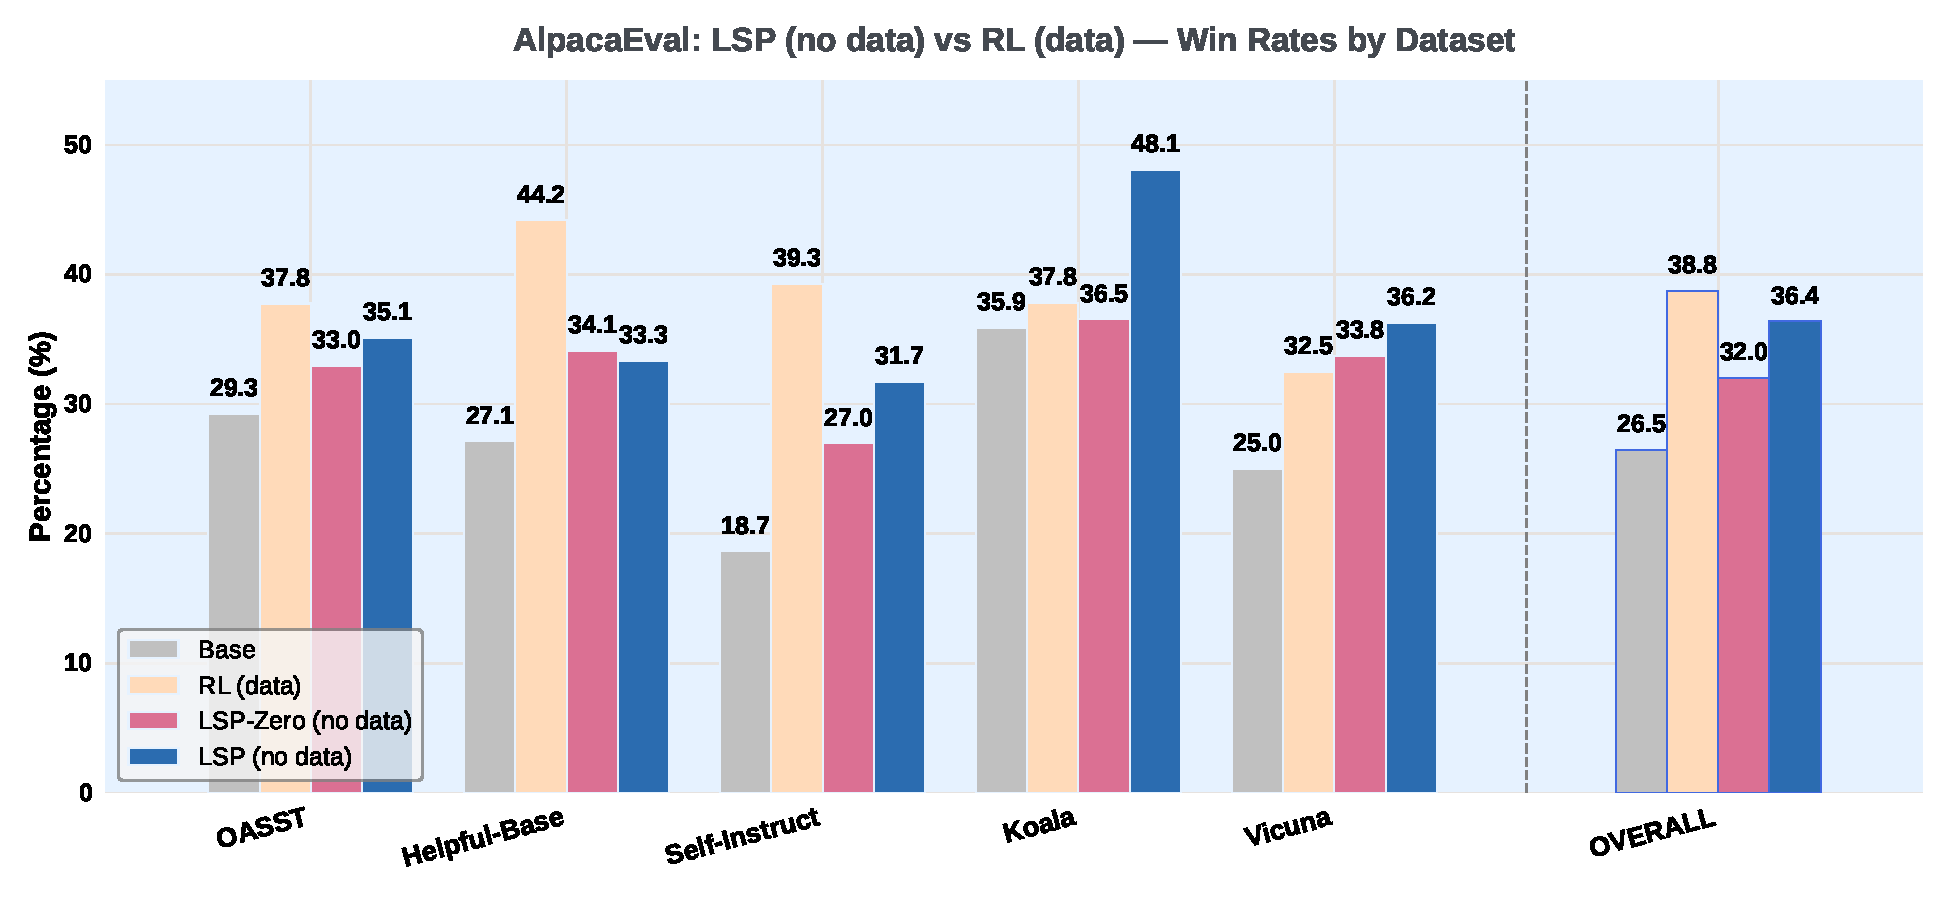
\includegraphics[width=\linewidth]{figures/lsp_vs_base.pdf}
    \caption{
        Comparison of win-rates of models trained with RL (GRPO, backed by data, yellow bars), 
        LSP-Zero and LSP (no data, red and blue bars, respectively) against the base model 
        (gray bars) on the AlpacaEval benchmark. 
        All algorithms improve upon the base model on the overall benchmark (right-most bars). 
        The overall win rates are: Base 26.5\%, RL 38.8\%, LSP-Zero 32.0\%, LSP 36.4\%.
    }
    \label{fig:alpaca-lsp-grpo-base}
\end{figure*}

After the release of the early version of this work, we learned about concurrent efforts that also conduct autonomous training that bear similarity to the challenger-solver one. 
Most notably, we found the works of \citet{zhao2025absolute}, \citet{chen2025self}, \citet{huang2025r}, and \citet{liu2025spiral}, particularly related.
The major differences between their and our algorithm ares: \emph{(1)} the query-generation step---unconstrained, viewed as a simple action in our case, and more carefully curated in those algorithms, and \emph{(2)} the rewarding mechanism, which in our case is a combination of a neural- and self-rewards while, in concurrent works, is based on majority-voting.
Thus, those methods specialize in tasks with deterministic, verifiable answers, while we welcome open-ended problems.
A synthesis of these paradigms is an important and exciting avenue of future work which we hope LSP to inspire.


\section{Experiments}
\label{sec:exp}
This section presents the empirical study of Language Self-Play. First, we carefully compare the effectiveness of \alz\ and \al\ on AlpacaEval Benchmark \citep{alpaca_eval}.
Then, we evaluate the main method of our paper, LSP, on standard LLM tasks.
Throughout the experiments, we use Llama-3.2-3B-Instruct \citep{dubey2024llama, meta2024llama32instruct} as the base model.
\subsection{The Importance of Self-Rewarding}

First, we compare data-free \al\ and, as ablation for the self-rewarding regularization, \alz\ to a model that was trained with RL from Alpaca data \citep{taori2023alpaca}.
The goal of that experiment is to analyze how much of performance of data-based training can be recovered with self-play alone in a scenario when RL data is fully missing.
In that setting, all models are initialized with the base model (Llama-3.2-3B-Instruct).
Then, we study the effectiveness of self-play as an intermediate stage between pre-training and data-based RL (LSP+RL).
Thus, in that experiment, we initialize our model with the model we obtained from self-play training in the first experiment.
Both experiments have an ablative role that evaluates the impotance of self-rewarding in \al.
All algorithms are evaluated with model sampling at $\tau=0.01$ temperature.
\begin{figure*}[t]
    \centering
    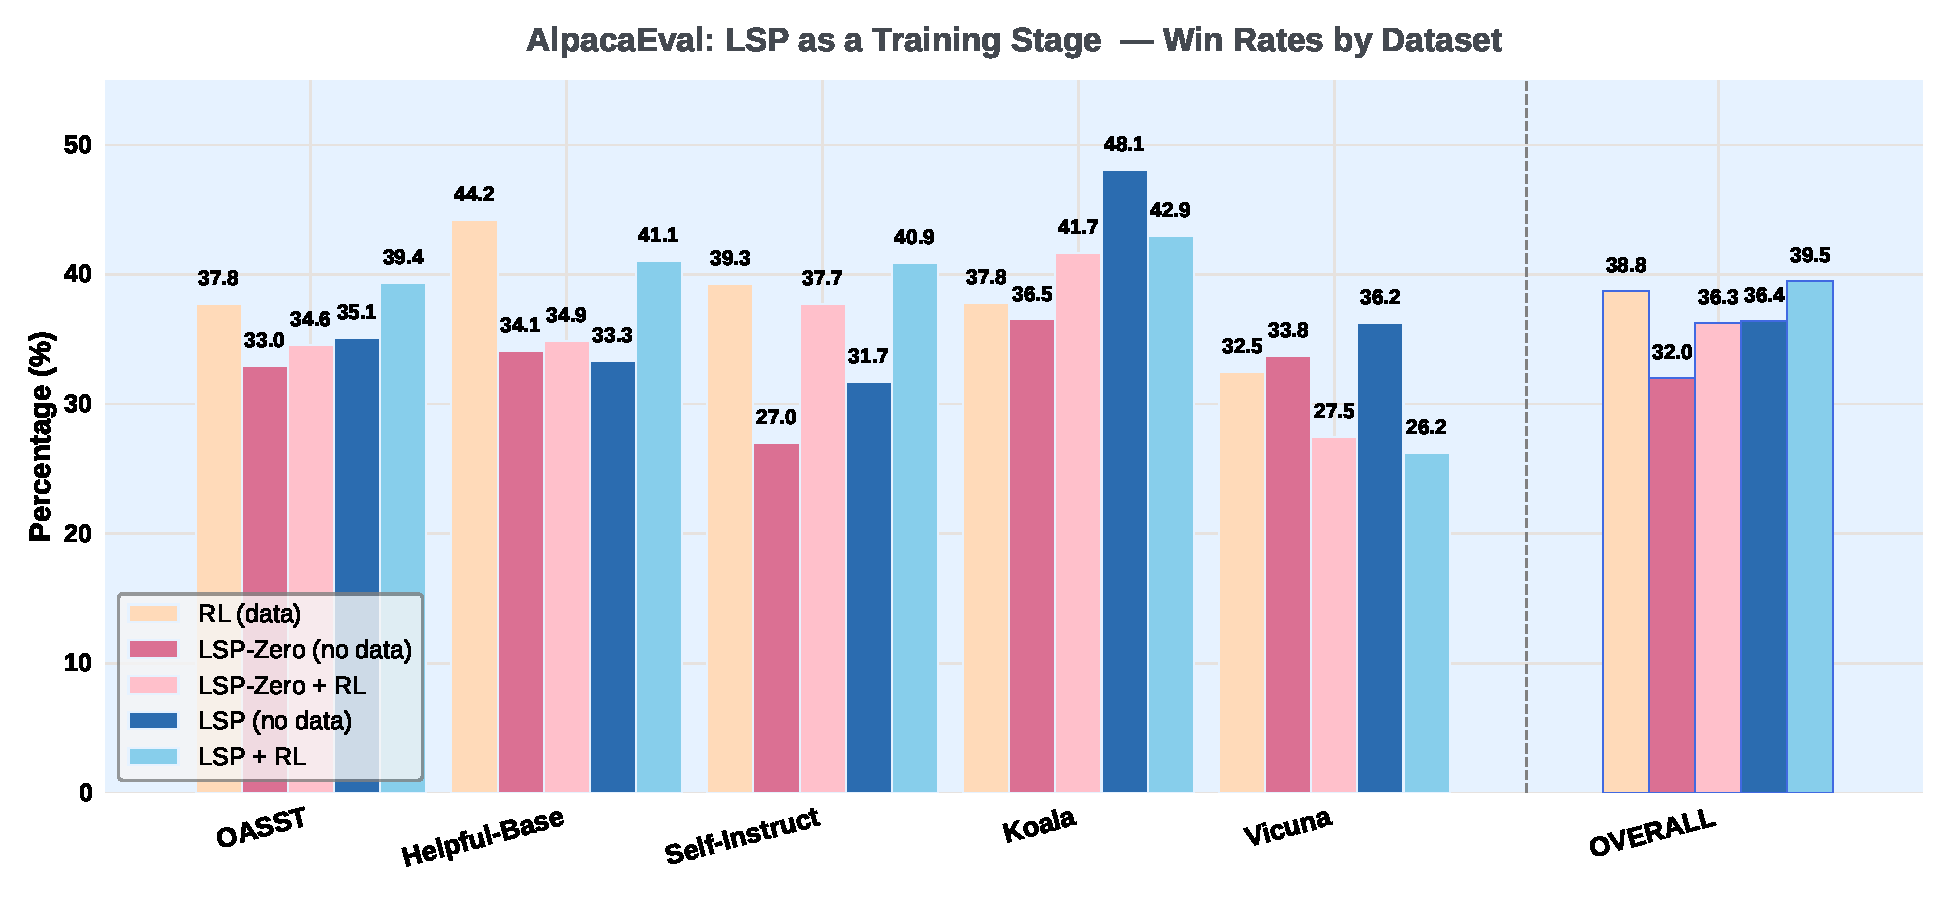
\includegraphics[width=\linewidth]{figures/lsp_vs_rl.pdf}
    \caption{Comparison of win-rates of the models trained with LSP-Zero and LSP (no data, red and blue bars), LSP-Zero and LSP, followed by RL (pink and light blue bars), and the model trained with GRPO only on AlpacaEval benchmark. 
    Further RL fine-tuning helps the self-play models, and the LSP+RL model achieves the best score. 
    The specific win rates are, RL 38.8\%, LSP-Zero 32.0\%, LSP-Zero+RL 36.3\%, LSP 36.4\%, and LSP+RL 39.5\%. }
    \label{fig:alpaca-lsp-grpo}
\end{figure*}
\paragraph{\textbf{Self-Play alone.}} In order to deliver interpretable results, as baselines, we compared our algorithms to the base model itself (Llama-3.2-3B-Instruct, \citep{dubey2024llama, meta2024llama32instruct}), as well as to one that we fine-tuned with traditional RL for LLMs that we instantiate with Group-Relative Policy Optimization \citep[GRPO]{shao2024deepseekmath}, whose implementation we obtained from HuggingFace's TRL library \citep{vonwerra2022trl}, on Alpaca training data \citep{taori2023alpaca}.
For all algorithms (GRPO, {\alz}, and {\al}), as a reward model, we used \emph{Skywork-Reward-V2-Llama-3.2-3B} \citep{liu2025skywork}\footnote{We note that in much of our algorithm development we utilized OpenAssistant's \emph{reward-model-deberta-v3-large-v2} but we found that, for all methods, the improved evaluation reward did not translate into improved AlpacaEval evaluation scores, while Skywork-Reward-V2 turned out to be very reliable.}.
For each of these algorithms, we calculate their win-rates against a copy of Llama-3.2-3B-Instruct on AlpacaEval (with Llama-4-Maverick as a judge), including results on each individual dataset, which we report in Figure \ref{fig:alpaca-lsp-grpo-base}.
The results show that \alz\ and \al\ effectively improve upon the base model, overall, in spite of not having used any training data.
In particular, \al\ achieves a similar overall result to GRPO.
%The experiment also reveals a greater effectiveness of LSP than that of LSP-Zero which we thus consider the main method proposed by this paper.
It is also worth noting that in some tasks, such as Koala---a dataset that specializes in conversational, open-ended instructions---\al\ ended up performing significantly better than the base model and GRPO.
This could be expected given that prompts generated by the challenger have such a character (see Box \ref{box:prompts}).

\paragraph{\textbf{Self-Play and RL.}}
Now, we initialize our models with the ones trained with \alz\ and \al\ in the previous experiment and train them with RL (GRPO).
Then, we calculate their win-rates against Llama-3.2-3B-Instruct and compare them to the plain RL model.
Th results from Figure \ref{fig:alpaca-lsp-grpo} show a significant improvement of \al\ (from 36.4\% to 39.5\%) of overall win-rate after further RL training.
Similarly, in this stage, \alz\ underperforms \al\---together with RL, it performs poorer overall than \al\ alone (36.3\% vs. 36.4\%).
Thus, this and the previous experiment lead us to consider \al\ as the main method of our paper.
\begin{comment}
Now, we initialize our model with the one trained with data-based RL (GRPO) in the previous experiment and train it with \alz\ and \al.
Then, we calculate its win-rates against Llama-3.2-3B-Instruct and compare them to the RL model we started from.
\begin{figure*}[t]
    \centering
    \includegraphics[width=\linewidth]{figures/lsp_vs_rl_new.pdf}
    \caption{Comparison of win-rates of the model trained with LSP-Zero and LSP (no data, red and blue bars) against the model it was initialized from - the model trained with GRPO (backed by data, yellow bars) on AlpacaEval benchmark. LSP performs better than GRPO overall and significantly better in Vicuna. The specific win rates are, GRPO 40.9\%, LSP-Zero 40.0\%, and LSP 43.1\%. 
    The solid gray line is the win-rate of the base model against itself.}
    \label{fig:alpaca-lsp-grpo}
\end{figure*}
Th results from Figure \ref{fig:alpaca-lsp-grpo} show a significant improvement of \al\ (from 40.9\% to 43.1\%) of overall win-rate (against Llama-3.2-3B-Instruct) after further self-play training.
Similarly to the previous experiment, the biggest gains can be observed in Vicuna where our algorithms improve GRPO's win-rate from 28.7\% to 36.3\% (\alz) and 46.3\% (\al).
However, in this stage, \alz\ has a negative net effect on the overall model performance further justifying the self-rewarding regularization. 
Thus, this and the previous experiment lead us to consider \al\ as the main method of our paper.
Also, admittedly, \al\ hinders the performance on some tasks, such as Koala, which is known to consist of chatbot user-type queries.
This is likely a consequence of our algorithm that biases its training queries to a structured, orderly style (see Boxes \ref{box:prompts} \& \ref{box:srp}).
Thus, making self-play robust by generating more diverse queries without damaging the model quality is an important avenue for future work.
\end{comment}

\begin{figure}
    \centering
    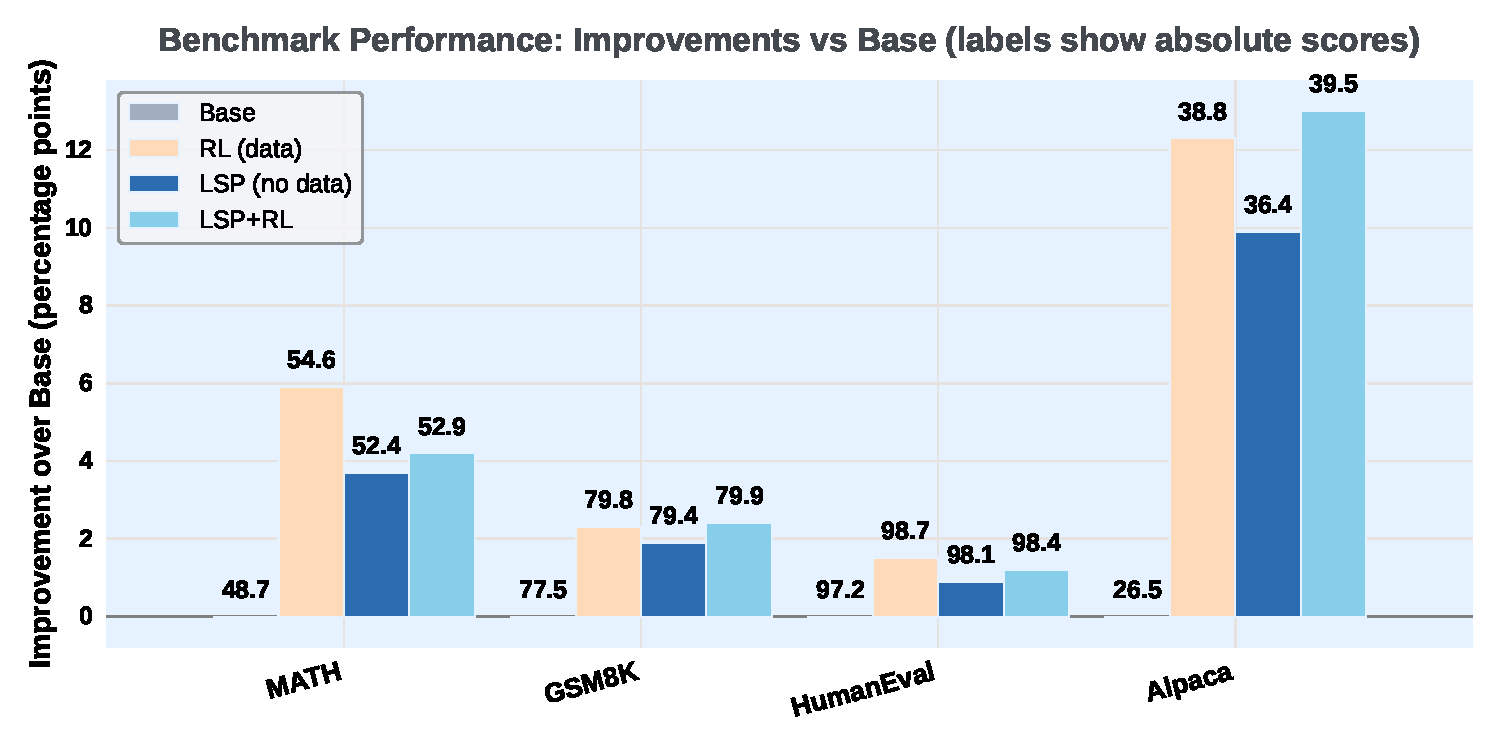
\includegraphics[width=\linewidth]{figures/benchmarks_improvement_over_base.pdf}
    \caption{Evaluation of the studied models on MATH, GSM8K, HumanEval, and Alpaca benchmarks.
    All the scores are graphically represented by bars of height of the absolute percent improvement over the base model, and labeled with the actual scores too.
    LSP (dark blue) recovers the majority of the improvement that RL (yellow) brings, and additional RL phase delivers even more improvement, making RL and LSP+RL better in different tasks.}
    \label{fig:all-evals}
    \vspace{-10pt}
\end{figure}
\subsection{Benchmark Evaluation of LSP}
We turn to comparing LSP, both as a standalone training procedure as well as an intermediate fine-tuning phase, to RL training with data represented by GRPO.
We utilize MATH \citep{hendrycks2021measuring}, GSM8K \citep{cobbe2021training}, HumanEval \citep{chen2021evaluating}, and Alpaca datasets \citep{alpaca_eval}.
Since MATH and GSM8K are both mathematics datasets, the standalone LSP is the same for both, trained with \emph{task='Pure \& Applied Mathematics'} in the challenger prompt (see Box \ref{box:chpt}).
We train GRPO on each dataset's training data, while evaluation takes place on the test set.
The exception is HumanEval which lacks a training set.
In its place, we use MBPP dataset \citep{austin2021program} for training.
The absolute improvement results in Figure \ref{fig:all-evals} demonstrate that the standalone LSP recovers \textbf{most of the performance} gains of GRPO, when trained from the pre-trained model, in spite of not having utilized data for training.
This result is significant because prior work notes that obtaining high-quality fine-tuning data is a key bottleneck for adapting LLMs—particularly for specialized use cases \citep{wang2022self, zhang2023instruction}.
It further shows that \al\ serves as an effective addition to RL fine-tuning from data in some tasks, although the gains are limited.
We suspect that this stems from the potential misalignment of the challenger-generated queries and the prompts given to the model at test time. 
This issue may persist to the RL phase (after LSP) via the KL-divergence constraint that prevents the learned model from diverging from the self-play model.
Closing this misalignment is an important avenue of future work.

\section{Conclusion}
In this work, we have offered a framework of perpetual improvement of a language model and the self-generated data that it learns from, as well as designed a practical algorithm---\emph{Language Self-Play} (LSP)---that enacts the framework given a pre-trained LLM. 
Our experiments confirm that LSP-Zero and LSP algorithms can improve pre-trained LLMs with no access to training data, especially on conversational tasks. 
While our experiments were conducted with preferential reward models, our algorithms can be just as well, if not easier, applied to problems with verifiable rewards.
In the case when verifiable ground-truth rewards are not readily available, the upper bound of the LSP model's performance is related to the judgement quality of the utilized reward model, as well as bounded by the human knowledge about the physical world. 
We believe, however, that such a self-play framework has a great potential to expand that knowledge once AI becomes embodied and capable of collecting its own empirical data.





\bibliographystyle{plainnat}
\bibliography{paper}

\clearpage
\beginappendix
\section{Example Plays}
\label{app:plays}
%\section{Responses To Challenger Prompts}
\begin{darkbluebox}{Challenger-Generated Prompts and Solver-Generated Responses}\label{box:responses}
    \begin{comment}
    \boxfont\textbf{Iteration 1.} {\color{BurntOrange}{Design a novel educational program to teach a 10-year-old child about the water cycle, incorporating a unique approach that combines storytelling with interactive games and activities to enhance engagement and understanding.}}
    \\
    \\
    {\boxfont\textbf{Iteration 150.} {\color{BurntOrange}Design a new line item in the menu for a futuristic space station that serves as a fusion of a high-end restaurant and a zero-gravity sports bar, and the item should be inspired by the culinary traditions of Japan and India.}}
    \\ 
    \\
    {\boxfont\textbf{Iteration 1500.} {\color{BurntOrange}Create a 10x10 grid and fill it with a chessboard setup where the white pieces are arranged in a specific pattern resembling a medieval knight's tournament formation, and include a chessboard to visualize the grid.}}
    \\
    \\
    {\boxfont\textbf{Iteration 2480.} {\color{BurntOrange}Design a ladder to reach the top of the Eiffel Tower using only a pair of high-quality ice skates and a teaspoon.}}
    \\
    \\
    \end{comment}
    \color{RoyalBlue}{
    %{\boxfont\textbf{Start.} {\color{BurntOrange} Design a novel educational program to teach a 10-year-old child about the water cycle, incorporating a unique approach that combines storytelling with interactive games and activities to enhance engagement and understanding.}} 
    %\\
    %\\
    {\boxfont\textbf{500 iterations.}\\ {\color{BurntOrange}Create a treasure map on a deserted island using a piece of paper, a pen, and two different rocks.}}
    \\
    {\boxfont\color{NavyBlue} \textbf{Treasure Map Creation Instructions}

\textbf{Materials}
\begin{itemize}\setlength\itemsep{0pt}
\item A piece of paper
\item A pen
\item Two different rocks
\end{itemize}

\textbf{Step 1: Choose a Location for the Coastline} \\
Find a suitable spot on the deserted island to mark the beginning of your treasure map. Use one of the rocks as a marker to indicate the starting point of your journey. A stick or a piece of driftwood may also be used as a makeshift marker.

\textbf{Step 2: Draw the Island's Shape} \\
Using the pen, draw a rough outline of the island's shape on the paper. Include notable features such as beaches, mountains, caves, and other landmarks. This should be a simplified representation rather than a geographically precise map.

\textbf{Step 3: Create a Grid System} \\
Draw a series of lines and squares on the paper to create a grid system. This helps plot coordinates and mark locations on the map. Divide the paper into smaller sections based on the desired level of detail. A $10 \times 10$ grid is a good starting point.

\textbf{Step 4: Plot the Treasure Location} \\
Using a different colored pen or pencil, choose a grid square and mark the treasure location with an \textbf{X}. Include directional information when needed, such as \emph{Due East} or \emph{North of the Mountain}.

\textbf{Step 5: Add Landmarks and Symbols} \\
Use the second rock to help define landmarks and symbols. For example:
\begin{itemize}\setlength\itemsep{0pt}
\item \textbf{X} for a rocky outcropping
\item A triangle for a cave entrance
\item Wavy lines for a stream or river
\end{itemize}
Use these symbols to mark notable landmarks and potential obstacles.

\textbf{Step 6: Add Additional Details} \\
Add further information such as water bodies (ocean waves, sea caves), weather patterns (sun, wind direction), hazard zones (cliffs, quicksand), and alternative routes or shortcuts.

\textbf{Step 7: Finalize and Review} \\
Review the map and make final adjustments. Ensure the map is easy to read and includes all necessary information. The second rock may also be used to create a mock navigation chart for future reference.
}
    % Exactly 490
    \newpage
    {\color{RoyalBlue}{\boxfont\textbf{1000 iterations.} \\
    \color{BurntOrange}Generate a set of instructions that an 5-year-old can follow to build a simple bridge using only 10 wooden blocks, a piece of string, and scissors, without a template or any external aid, within a 10-minute time frame. }}
    % Exactly 990
    \\
    {\color{NavyBlue}Here is a step-by-step guide to build a simple bridge using 10 wooden blocks, a piece of string, and scissors that a 5-year-old can follow.

\textbf{Step 1: Get Ready!} \\
Find a flat and clear space to play. Place the wooden blocks so they are standing upright. Take the piece of string and cut it into two or three equal pieces, depending on how big you want the bridge to be.

\textbf{Step 2: Build the Base} \\
Choose six blocks and stack them side by side to create the base of the bridge. Make sure the blocks are snug together and stable.

\textbf{Step 3: Create the Supports} \\
Choose two blocks and place them on either side of the base, about one block apart. Bend the string into a gentle curve and attach one end to the top of each support block. Pull the string taut so it is stretched out.

\textbf{Step 4: Add the Sides} \\
Take the remaining two blocks and place them side by side, parallel to the supports. Bend the string around the blocks, making sure it is not too tight or too loose. Adjust the tension by gently pulling the string.

\textbf{Step 5: Secure the Bridge} \\
Take the last two blocks and place them on top of the supports, one on each side. Bend the string around the blocks again to hold everything in place.

\textbf{Step 6: Test Your Bridge!} \\
Gently try walking across the bridge and check that it feels sturdy.

\textbf{Tips and Reminders} \\
Always ask an adult for help if you are unsure about something. Be careful not to knock over the blocks or the bridge while building or playing. Do not pull the string too hard, or the bridge may break.

\textbf{Time's Up!} \\
You did it! You built a simple bridge using just 10 wooden blocks, a piece of string, and scissors. Practice makes perfect, so try building another one soon.
}
    \\
    \\

\newpage
{\color{RoyalBlue}\boxfont\textbf{1500 iterations.} \\
{\color{BurntOrange}Write a 2048-line assembly code for a subtracting two 16-bit numbers stored in two consecutive 32-bit registers. The numbers should be stored in the registers and the result should be automatically saved in a new register.} 

Here is a high-level assembly example for subtracting two 16-bit numbers stored in two consecutive 32-bit registers.

\textbf{Note} \\
The code is written in a way that can be easily modified to suit different architectures.

\textbf{Assumptions}
\begin{itemize}\setlength\itemsep{0pt}
\item A 32-bit architecture is used.
\item The numbers are signed 16-bit values (two's complement representation).
\item All registers are 32-bit wide.
\end{itemize}

\textbf{Assembly Code}

\begin{verbatim}
; subtract_two.asm

    ; Register declarations
    MOV AX, 0     ; AX stores the first 16-bit number
    MOV CX, 0     ; CX stores the second 16-bit number
    MOV DX, 0     ; DX stores the result

    ; Subtract the two numbers
    SUB AX, CX    ; AX = AX - CX

    ; After subtraction, AX holds the result
    ; If the result is negative, compute two's complement
    JSUB AX, 0    ; JSUB performs two's complement conversion

    ; Move the result to DX
    MOV DX, AX

    ; Optional output code
    ; MOV AH, 09h
    ; INT 21h

    ; Adjust for sign extension
    SHR DX, 1
    ADD DX, DX
    JZ SUB_done

    ; If sign bit is set, subtract 2^16
    SUB DX, 0xFFFF

SUB_done:
    ; Final result is in DX
\end{verbatim}

\textbf{Important Note} \\
Direct subtraction using two's complement arithmetic in assembly does not behave the same way as decimal subtraction, and sign handling must be done explicitly when working with smaller word sizes.
    
 }}
    % Exactly 1510
\end{darkbluebox}

\section{An Example Of Unregularized Play}
\label{appendix:ufo}
\begin{darkbluebox}{Challenger-Generated Prompts and Solver-Generated Responses}
\label{box:ufo}
\color{RoyalBlue}{
{\small\color{BurntOrange}
A large, unidentified object is seen in a distance. Describe the object's physical properties and suggest possible uses for it, but do not describe its name.
}
{\small
\begin{verbatim}
class UnidentifiedObject:
    def __init__(self):
        self.properties = ["size", "shape", "material", "color", "origin"]
        self.possibilities = ["ancient relic", "spacecraft",
                              "natural formation", "alien artifact"]
    def describe(self):
        self.size = ["large", "small"]
        self.shape = ["cylindrical", "spherical", "irregular"]
        self.material = ["metal", "stone", "wood", "carbon fiber"]
        self.color = ["black", "white", "gray", "silver"]
    def analyze(self):
        raise NotImplementedError
    def suggest_possibilities(self):
        raise NotImplementedError
    def draw(self):
        raise NotImplementedError
    def identify(self):
        self.possibilities = ["possible uses"]
    def evaluate(self):
        self.suggest_possibilities(self.possibilities())

class UnknownObject(UnidentifiedObject):
    def __init__(self):
        super().__init__()
        self.origin = ["unknown", "mysterious", "cosmic"]
    def analyze(self):
        self.properties["size"] = self.size()
        self.properties["shape"] = self.shape()
        self.properties["material"] = self.material()
    def draw(self):
        print("Drawing the object...")
        self.draw()
    def suggest(self):
        self.identify()
        self.suggest_possibilities()
    def evaluate(self):
        self.suggest()
        self.draw()

def main():
    obj = UnknownObject()
    obj.describe()
    obj.analyze()
    obj.suggest()
    obj.draw()

if __name__ == "__main__":
    main()
\end{verbatim}
}
}
\end{darkbluebox}

\section{Hyper-parameters}

\begin{table}
\centering
\begin{tabular}{lcccccc}
\hline
Method & \#queries & $\beta$ & Self-Reward & Learning rate & n.grad.acc. & Batch size \\
\hline
GRPO & 8 & 0.05 & No & $1\times10^{-6}$ & 2  & 4 \\
LSP-Zero   & 8 & 0.05 & No & $3\times10^{-6}$ & 2  & 4  \\
LSP  & 8 & 0.05 & Yes & $3\times10^{-6}$ & 2 &  4  \\
\hline
\end{tabular}
\label{tab:hyperparams-grpo}
\caption{Hyper-parameters used for training with GRPO, LSP-Zero, and LSP algorithms.}
\end{table}

\end{document}
